\documentclass{beamer}
\usepackage{cmap}
\usepackage[T1]{fontenc}
\usepackage[french]{babel}
\usepackage{microtype}
\usepackage{url, hyperref}
\usepackage{graphicx}
\usepackage{emoji}

\usetheme{Dresden}

\setbeamertemplate{navigation symbols}{}

\definecolor{purple}{rgb}{0.5, 0, 1}
\setbeamercolor*{palette primary}{use=structure, fg=white, bg=purple}
\setbeamercolor*{palette secondary}{use=structure, fg=white, bg=purple}
\setbeamercolor*{palette tertiary}{use=structure, fg=white, bg=purple}
\setbeamercolor*{palette quaternary}{use=structure, fg=white, bg=purple}

\setbeamercolor*{sidebar}{fg=purple,bg=gray!15!white}

\setbeamercolor*{palette sidebar primary}{fg=purple!10!black}
\setbeamercolor*{palette sidebar secondary}{fg=white}
\setbeamercolor*{palette sidebar tertiary}{fg=purple!50!black}
\setbeamercolor*{palette sidebar quaternary}{fg=gray!10!white}

\setbeamercolor{titlelike}{parent=palette primary,bg=purple}
\setbeamercolor{frametitle}{bg=yellow!90!white, fg=purple}
\setbeamercolor{frametitle right}{bg=gray!60!white}

\title{CPU et horloge sur FPGA}
\author[%
J. \textsc{Caspar},
L. \textsc{Chevalier},
V. \textsc{Ivanov},
A. \textsc{Mathieu}%
]{
  Jean \textsc{Caspar},
  Loïc \textsc{Chevalier},
  Vladimir \textsc{Ivanov},
  Adrien \textsc{Mathieu}
}
\date{24 Janvier 2023}

\begin{document}

\begin{frame}[noframenumbering]
  \titlepage
\end{frame}

\begin{frame}[fragile]{Jeu d'instructions}
  L'instruction set de notre CPU est inspiré de RISC-V. Chaque
  instruction peut prendre un ou deux arguments, et éventuellement
  spécifier un registre où stocker le résultat.\par
  \pause
  16 registres 16-bit sont disponibles. Le premier, \(r_0\), vaut
  toujours \(0\).\par
  \pause
\end{frame}

\begin{frame}[fragile]{Familles d'instructions}
  Les instructions disponibles se divisent en quatre familles\pause
  \begin{itemize}
  \item Les opérations arithmétiques et logiques. Celles-ci incluent
    la division et le modulo, mais ne sont pas utilisées dans notre
    programme.
    \pause
  \item Les opérations de comparaison. Elles se déclinent en opérations
    signées et non-signées. Toutes les opérations ne sont pas
    disponibles (manque de place).
    \pause
  \item Les opérations de saut. Les sauts relatifs sont supportés, mais
    jamais utilisés.
    \pause
  \item Les opérations externes à la CPU. Cela correspond à la RAM et
    aux ports d'IO.
  \end{itemize}
\end{frame}

\begin{frame}{Assembleur}
  Un assembleur\footnote{\emoji{crab}} est fourni avec la CPU. En plus
  de simplement assembler, il permet quelques facilités, qui ne sont
  que du sucre syntaxique.\par
  \pause
  Par exemple, toutes les opérations de comparaison sont disponibles
  dans l'assembly; elles sont ensuite exprimées en fonction de celles
  disponibles.\par
  \pause
  De même, la RAM et les ports d'IO peuvent être utilisés comme un
  tableau en C, et les expressions arithmétiques sont résolues au
  moment de la compilation en un immédiat unique.
\end{frame}

\begin{frame}{Verilog}
    Le programme Verilog est séparé en plusieurs modules.
    \begin{itemize}
        \item ALU et comparateur
        \item Un pointeur d'instruction, et un module pour gérer les sauts
        \item Des registres, de la RAM et un sélecteur d'instruction
        \item Des bus et un module de gestion de l'IO
        \item Un driver qui instancie les autres modules
    \end{itemize}
\end{frame}

\begin{frame}{VM}
    \begin{itemize}
        \item VM qui simule les opérations du CPU
        \item Peut prendre en paramètre la fréquence à laquelle simuler, l'état des registres (y compris l'addresse de l'instruction courante)
        \item Peut afficher l'état interne du CPU virtuel à chaque cycle
        \item Gestion des I/O séparée du c\oe{}ur de la VM : programmes de tests sans entrée/sortie contre programme de l'horloge avec des entrées/sorties spécifiques
    \end{itemize}
\end{frame}

\begin{frame}{Simulateur}
    \begin{itemize}
        \item Simule le CPU physique
        \item Par défaut, exécute aussi vite que possible ; wrapper Python autour ainsi qu'une légère modification du code du CPU non synthétisable pour forcer l'horloge à être à la fréquence attendue
        \item Dernière étape avant le téléchargement sur le FPGA
    \end{itemize}
\end{frame}

\begin{frame}[fragile]{Programme}
    \begin{itemize}
        \item Horloge : de secondes à année
        \item Deux phases :
            \begin{enumerate}
            \item initialisation, déplacement entre des boucles selon les entrées de l'utilisateur
            \item boucle principale, deux registres utilisés pour retenir le nombre de cycles écoulés ($12 \cdot 10^6 = 183 \cdot 2^16 + 6912$)
            \end{enumerate}

        \item Gestion des jours : utilisation d'un registre pour ne pas recalculer le dernier jour du mois tous les jours (seulement tous les mois)
        \item Gestion des années bissextiles : utilisation de 3 registres pour repérer quelle année modulo 400 on est sans utiliser de division ou de modulo, utilisation d'un registre pour mémoriser cette information (en fait \verb+r11+ retient le nombre de jour au mois de février)
    \end{itemize}
\end{frame}

\begin{frame}{FPGA}
    Précédemment nous avions tenté d'utiliser 12 afficheurs 7 segments pour tout afficher en même temps.
    Mais le FPGA n'a pas autant de sorties donc il aurait fallu utiliser des puces en plus pour servir
    de registres et de décodeur.
    \begin{center}
        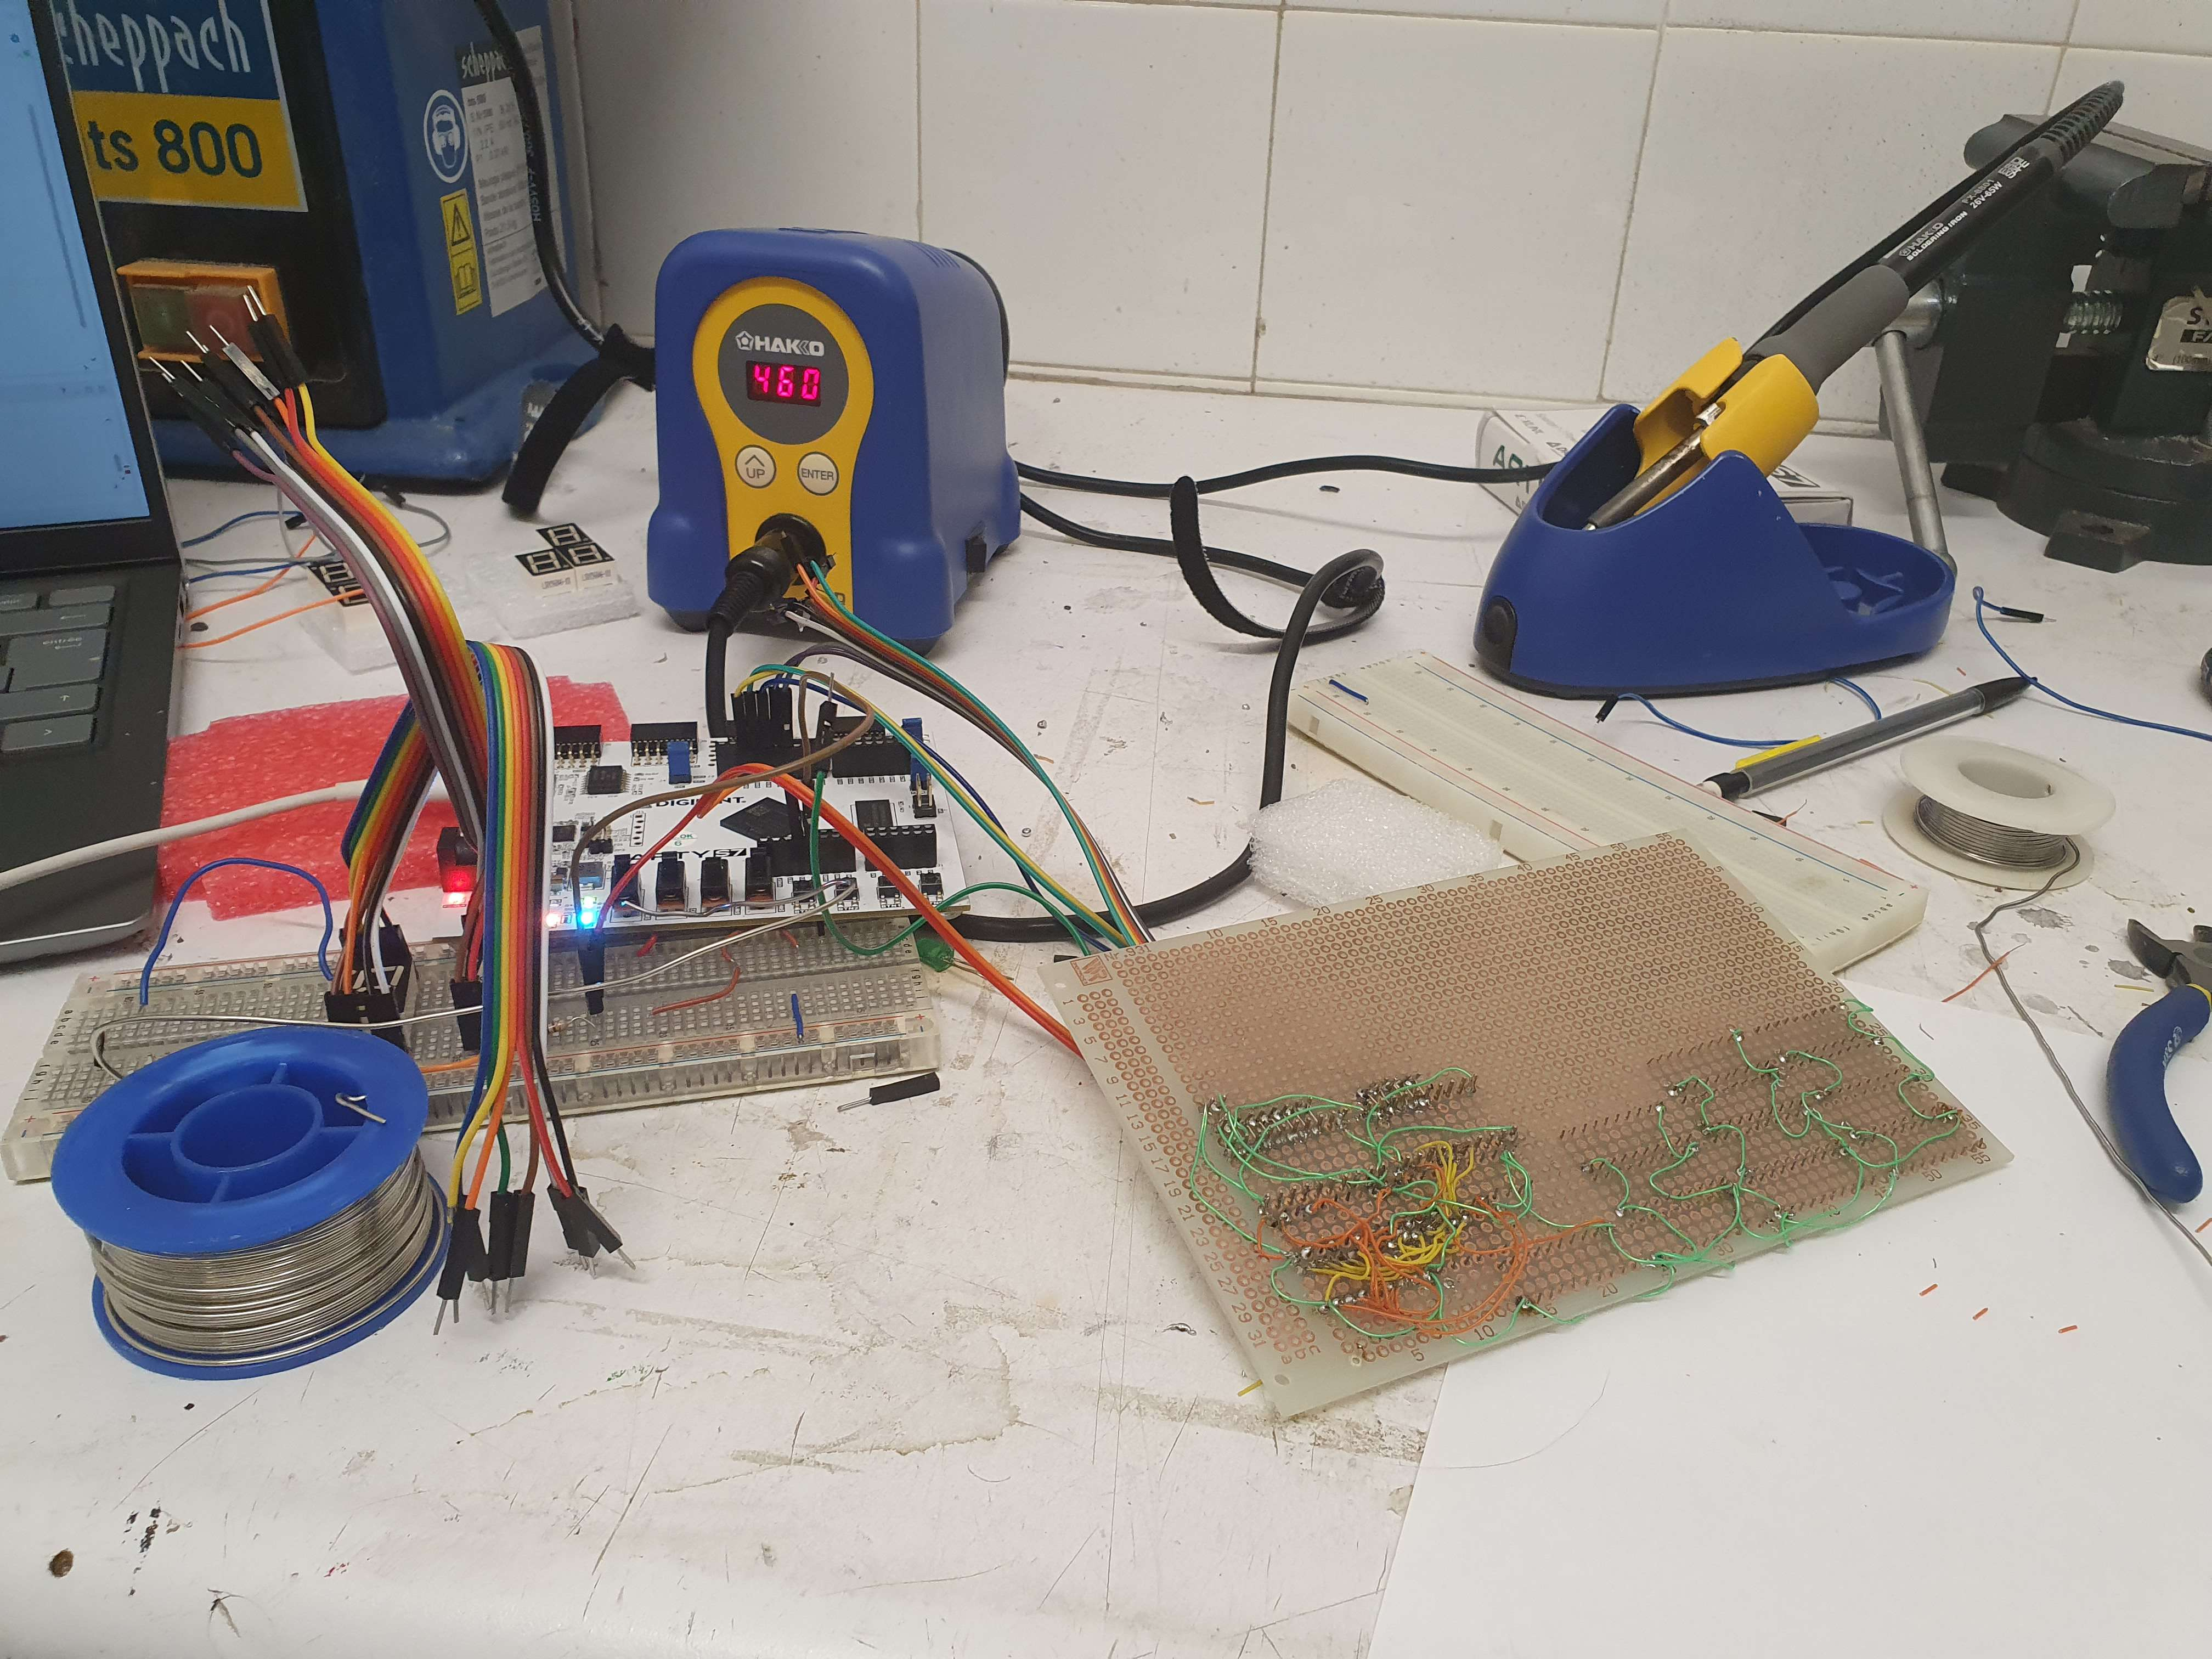
\includegraphics[scale=0.05]{pictures/Soudure global.jpg}
    \end{center}
\end{frame}

\begin{frame}
    C'est un échec :
    \begin{center}
        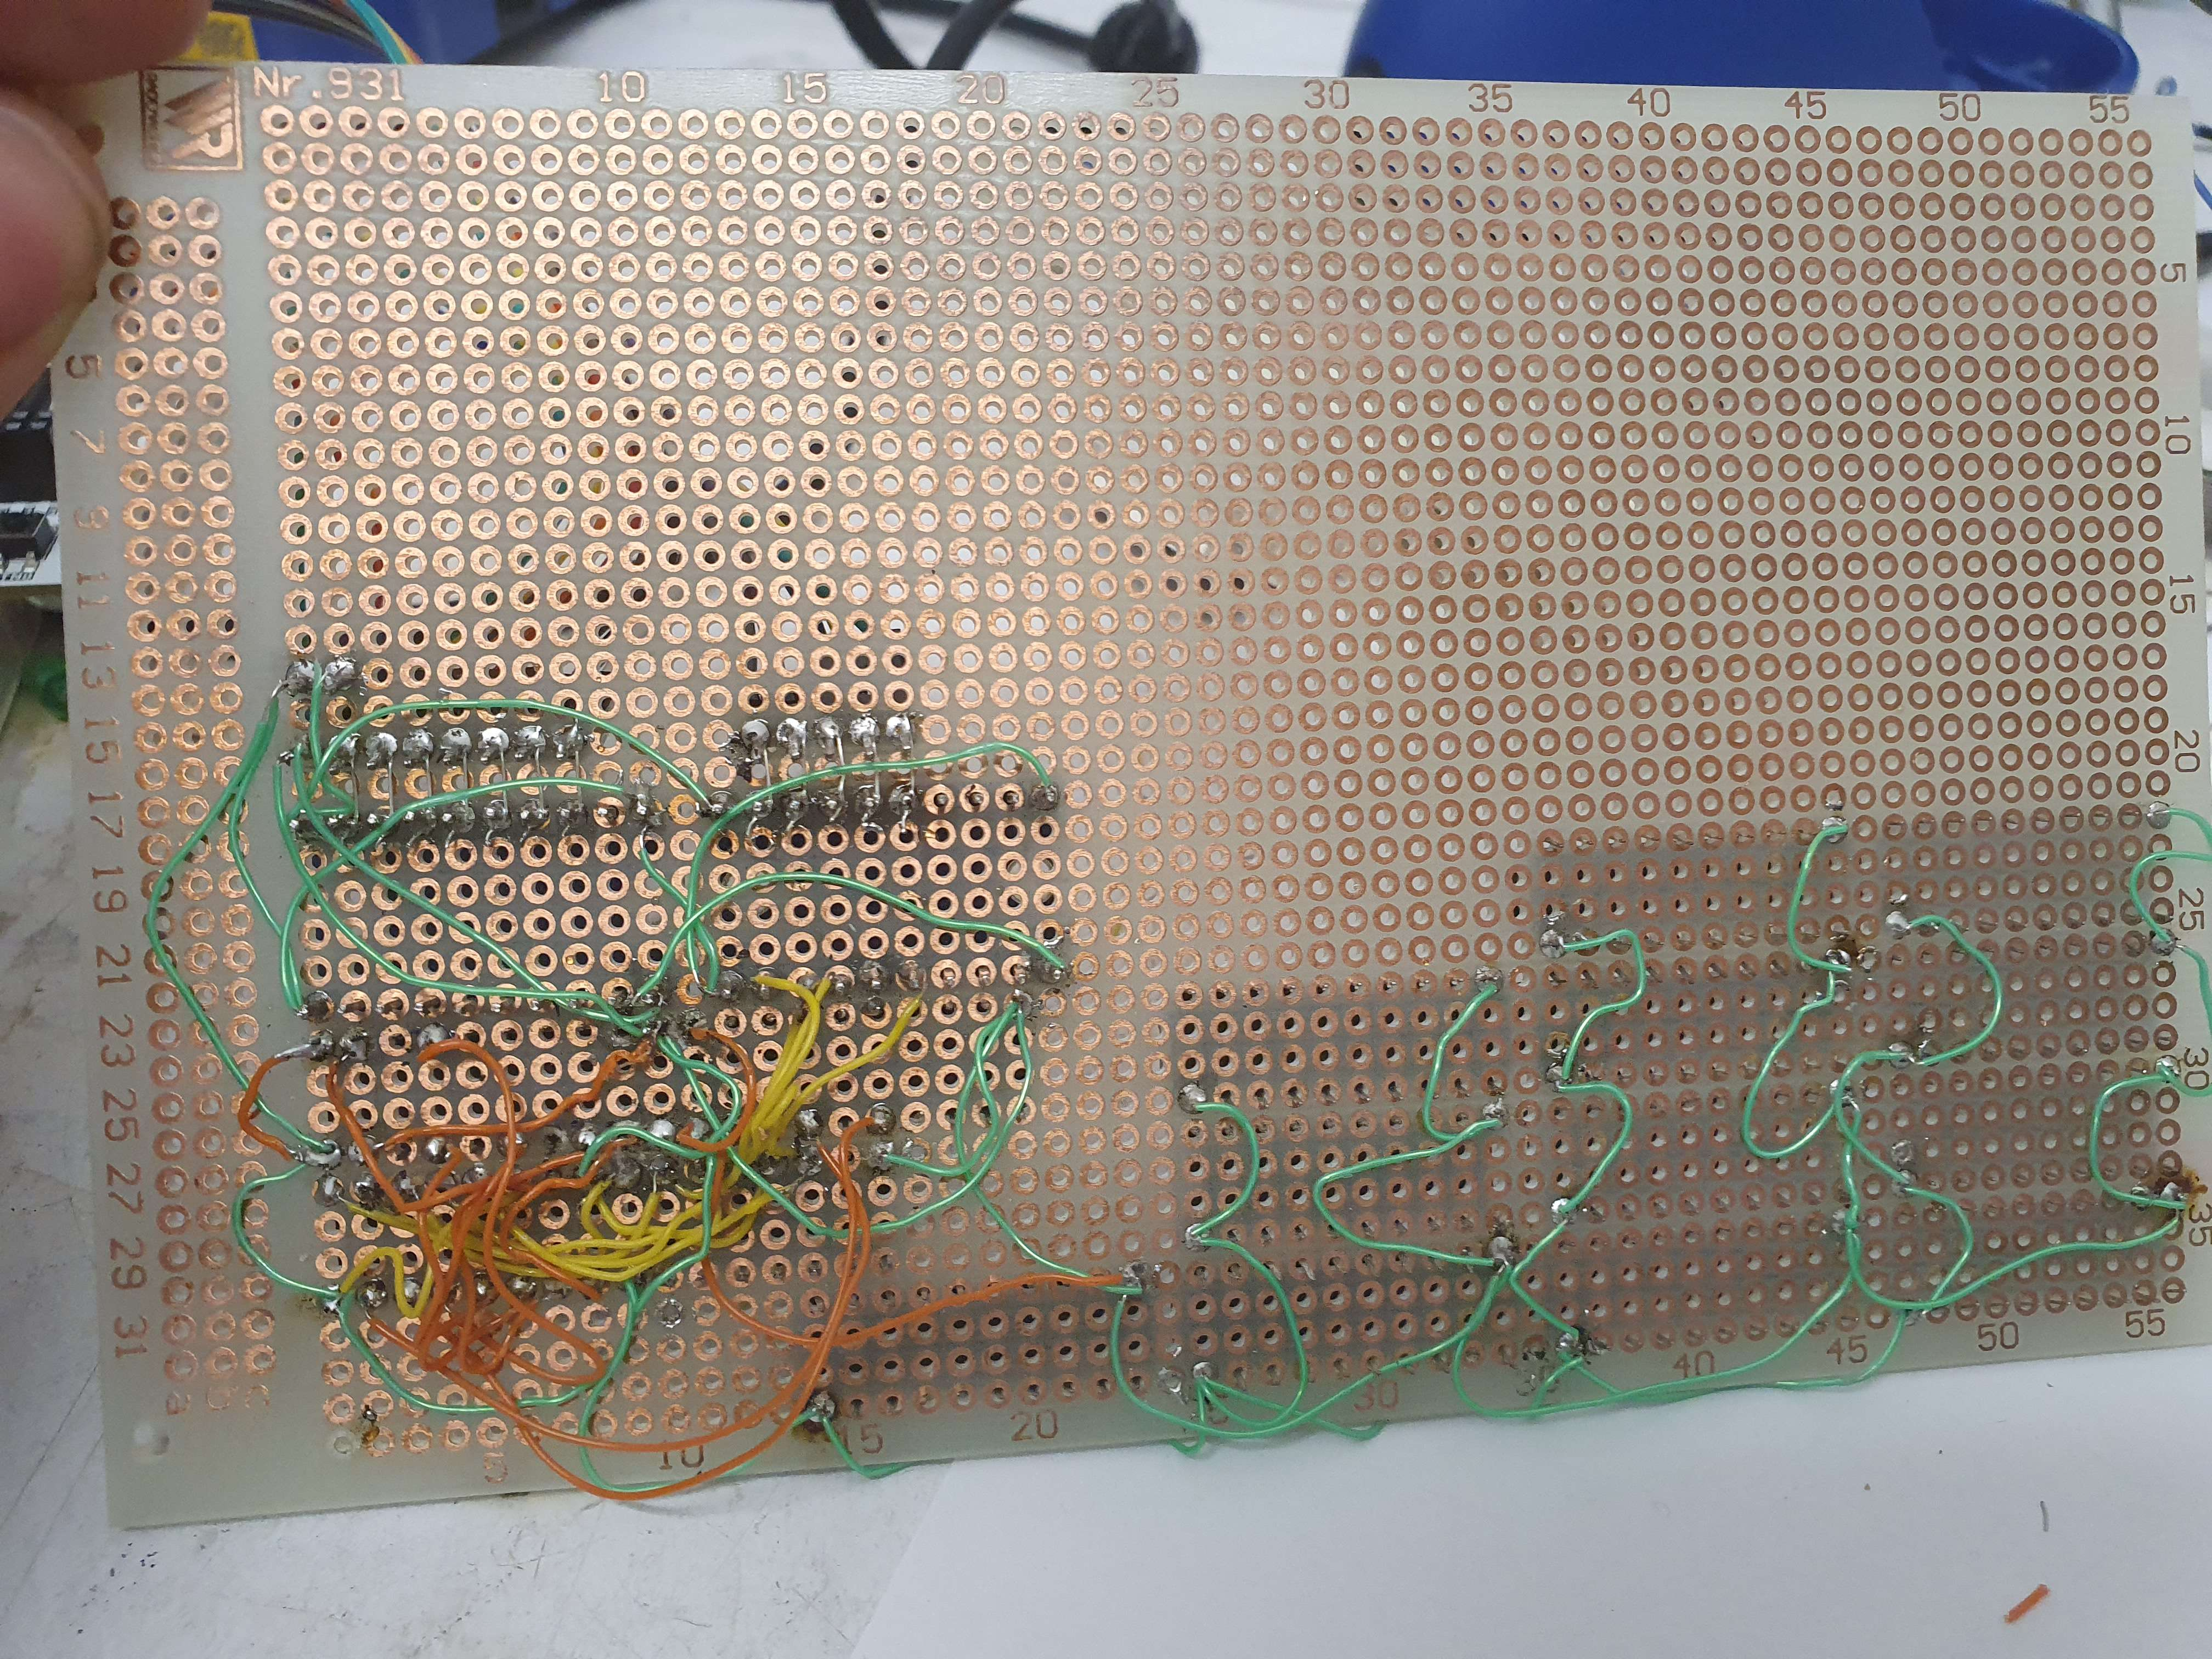
\includegraphics[scale=0.07]{pictures/Soudure proche.jpg}
    \end{center}
\end{frame}

\begin{frame}
    Nous sommes mauvais en soudure, et il y avait trop de court-circuit, donc nous avons abandonné.
    Finalement, nous avons utilisé une breadboard (pas besoin de soudures) et seulement 6 afficheurs,
    on peut changer de mode d'affichage avec les boutons. Nous pouvons afficher HH/MM/SS, YY/MO/DD
    ou YYYY/MO.
    \begin{center}
        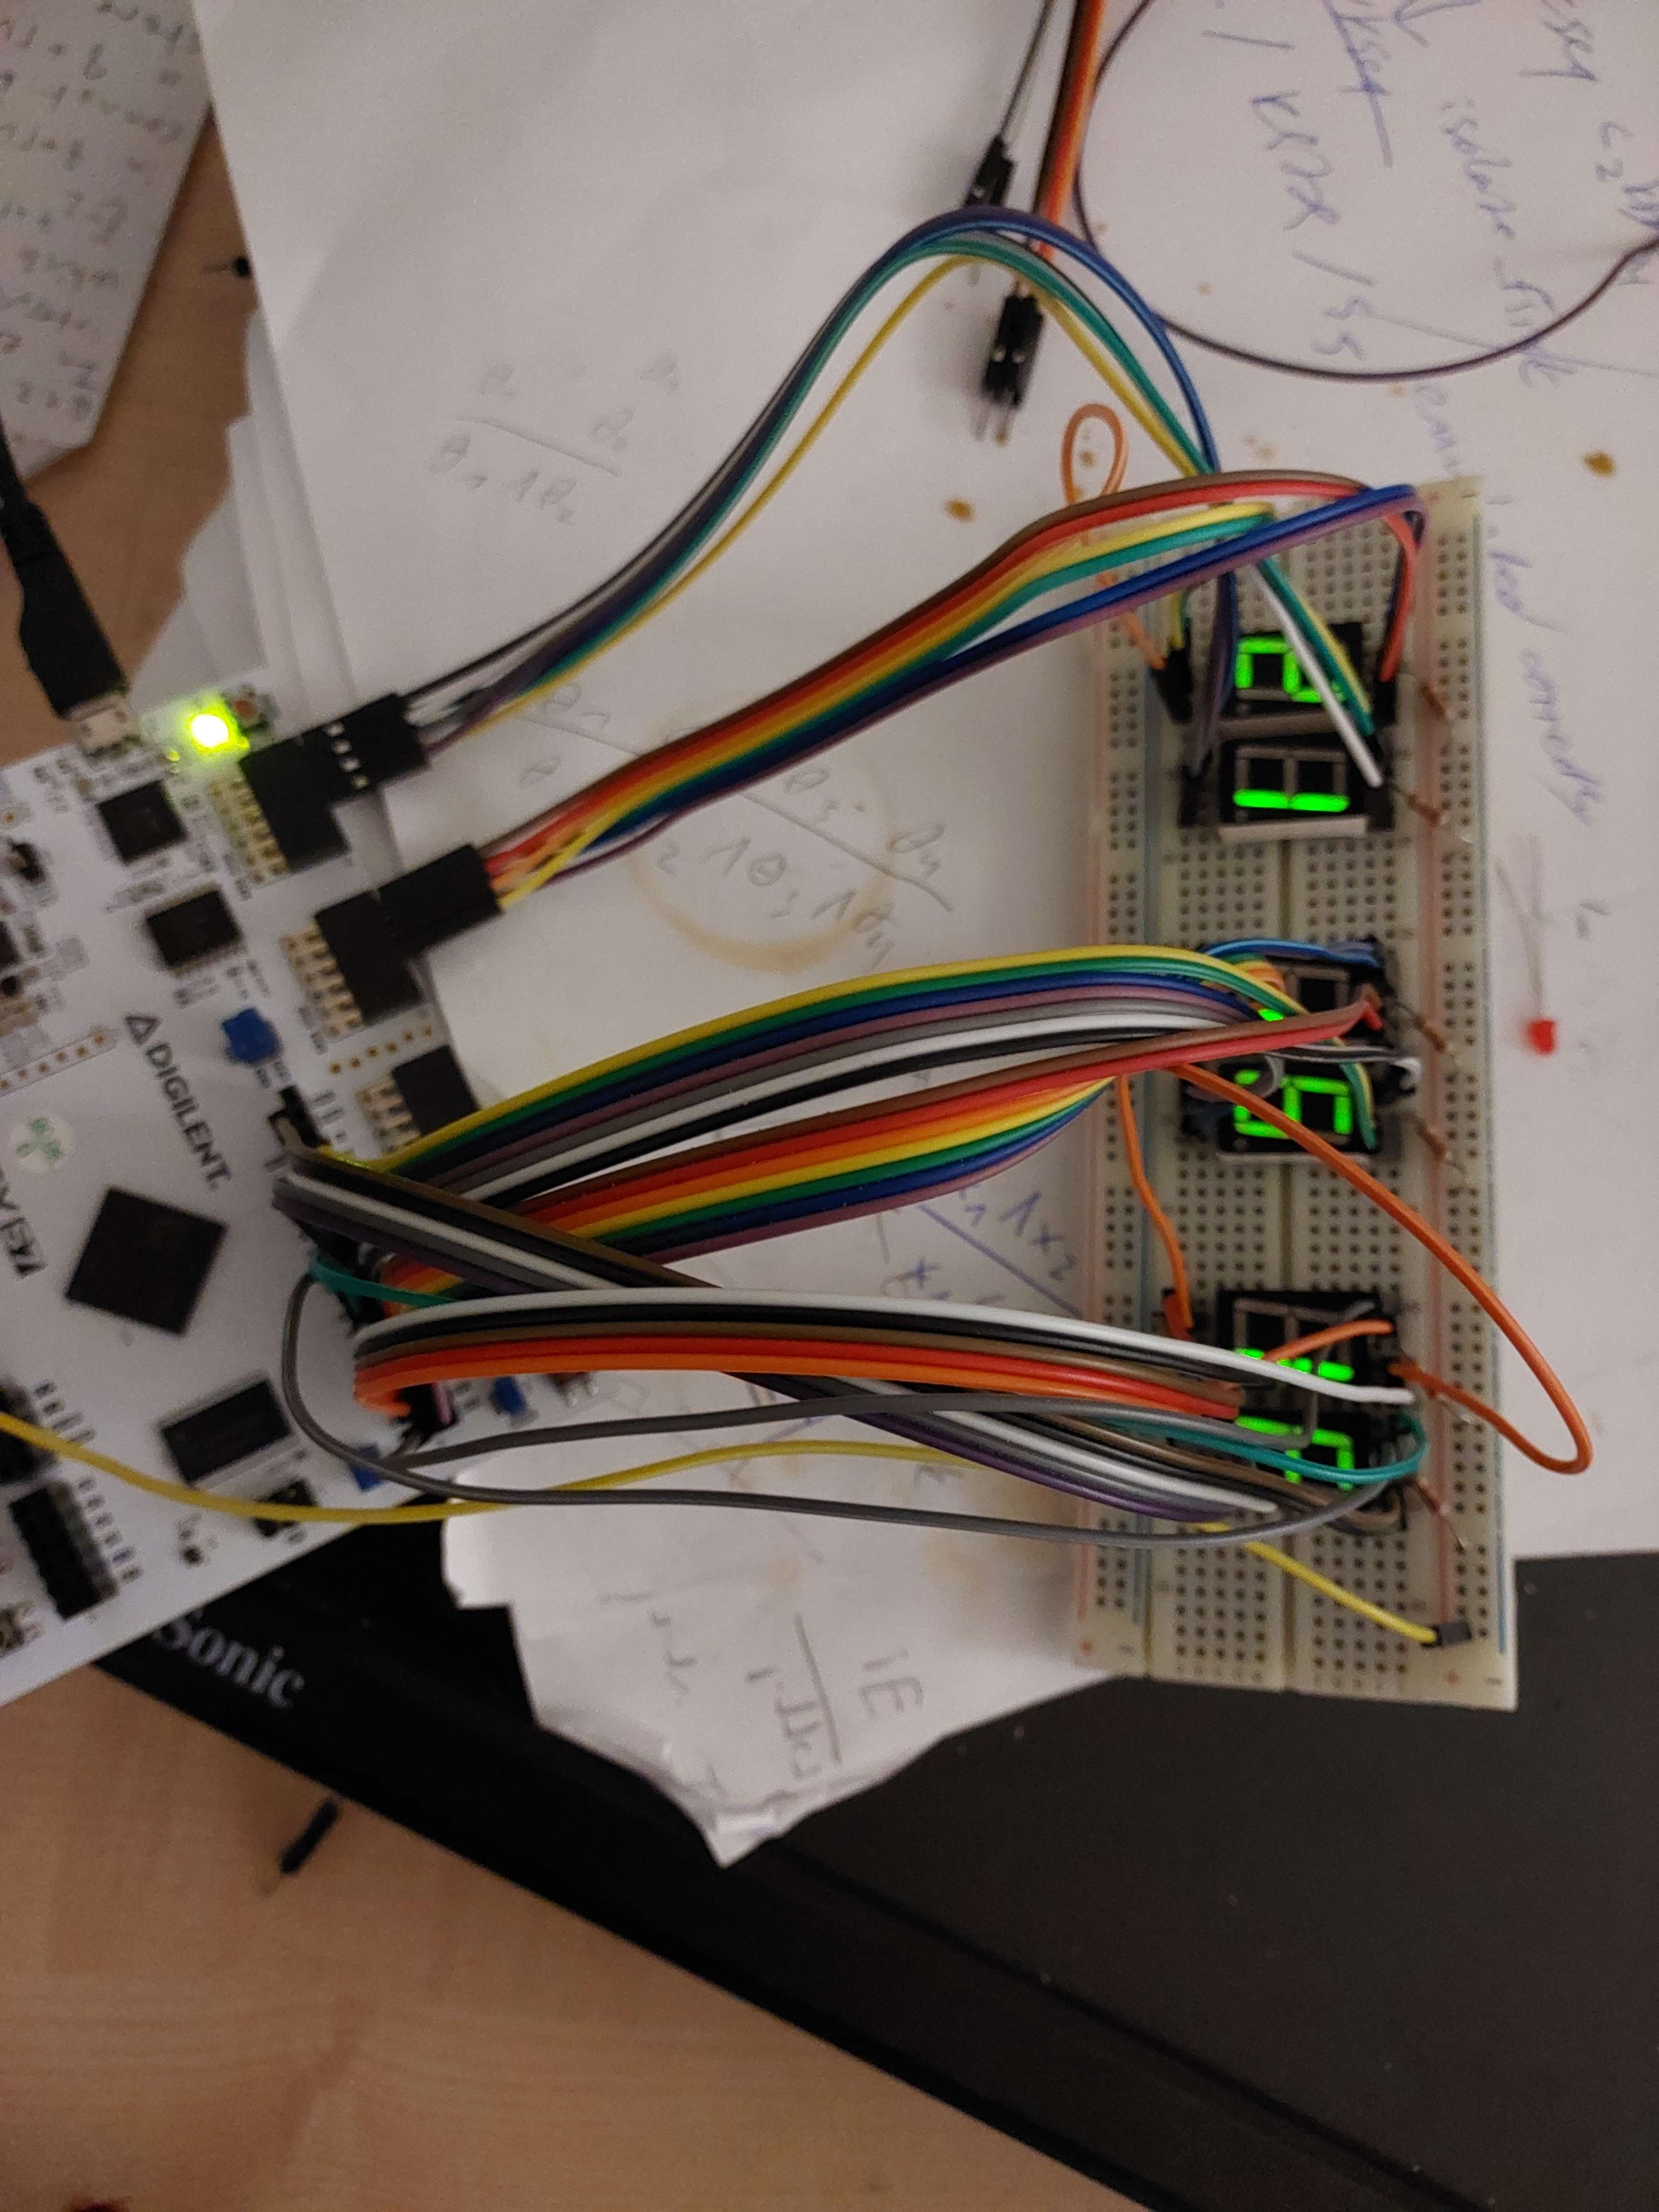
\includegraphics[angle=90,scale=0.04]{pictures/FPGA final.jpg}
    \end{center}
\end{frame}

\end{document}
